\begin{figure}[H]
  \centering
  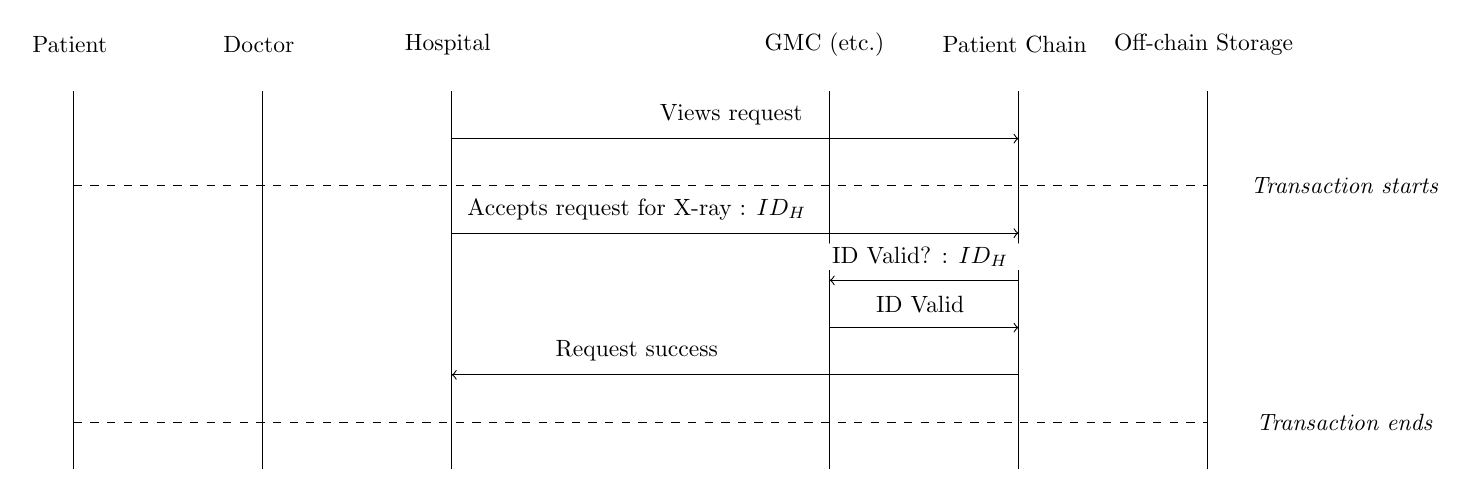
\begin{tikzpicture}[scale = 0.6, every node/.style={scale = 0.85}, every node/.append style={fill = white, rounded corners = 2pt, inner sep = 2pt, align = center}]

  % Lines
  \draw (4, 12) -- (4, 20);
  \draw (8, 12) -- (8, 20);
  \draw (12, 12) -- (12, 20);
  \draw (20, 12) -- (20, 20);
  \draw (24, 12) -- (24, 20);
  \draw (28, 12) -- (28, 20);

  % Headings
  \node at (4, 21) { Patient };
  \node at (8, 21) { Doctor };
  \node at (12, 21) { Hospital };
  \node at (20, 21) { GMC (etc.) };
  \node at (24, 21) { Patient Chain };
  \node at (28, 21) { Off-chain Storage };

  % Arrows
  \node at (18, 19.5) { Views request };
  \draw [ -> ] (12, 19) -- (24, 19);

  \node at (31, 18) { \textit{Transaction starts} };
  \draw [ dashed ] (4, 18) -- (28, 18);

  \node at (16, 17.5) { Accepts request for X-ray : $ID_{H}$ };
  \draw [ -> ] (12, 17) -- (24, 17);

  \node at (22, 16.5) { ID Valid? : $ID_{H}$ };
  \draw [ -> ] (24, 16) -- (20, 16);

  \node at (22, 15.5) { ID Valid \checkmark };
  \draw [ -> ] (20, 15) -- (24, 15);

  \node at (16, 14.5) { Request success };
  \draw [ -> ] (24, 14) -- (12, 14);

  \node at (31, 13) { \textit{Transaction ends} };
  \draw [ dashed ] (4, 13) -- (28, 13);

  \end{tikzpicture}
  \caption{Hospital accepts a doctor's request for an X-ray}{
    The hospital accepts the request, made by the doctor, for the patient's X-ray. This paves the way for the hospital and the patient to negotiate a time for the appointment. \textit{Note: whilst the hospital is shown as having some $ID_{H}$ above, in reality this might be the id of an administrator of X-ray requests who is a member of a hospital administration group (similar to the GMC for doctors).}
  }
  \label{fig:user_story_01b}
\end{figure}
